\documentclass[12pt]{article}

\usepackage{tikz}

\usepackage{pgfplots}

\begin{document}

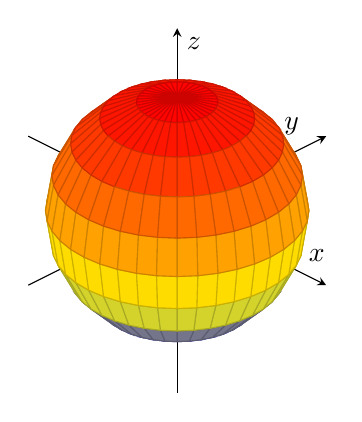
\begin{tikzpicture}
\begin{axis}[%
        axis equal,
        width=10cm,
        height=10cm,
        axis lines = center,
        xlabel = {$x$},
        ylabel = {$y$},
        zlabel = {$z$},
        ticks=none,
        enlargelimits=0.3,
        view/h=45,
        scale uniformly strategy=units only,
    ]
\addplot3[%
        opacity = 1,
        surf,
        z buffer = sort,
        samples = 21,
        variable = \u,
        variable y = \v,
        domain = 0:180,
        y domain = 0:360,
    ]
    ({cos(u)*sin(v)}, {sin(u)*sin(v)}, {cos(v)});
    \end{axis}
    
    
%	\draw[<->] (-2, 0) -- (2, 0);
%	\draw[<->] (0, -2) -- (0, 2);
%	
%    \shadedraw[shading=ball,ball color=purple, white] (0.0,0) circle (1.5);
%
% \pgfmathsetmacro\tell{-sin(20)}
%    \pgfmathsetmacro\bell{sin(20)}
%    \pgfmathsetmacro\rell{1.5 * sin(20)}
%    \begin{scope}
%        \clip (0,0) +(-1.5,0) arc (-180:0:1.5 and 1.5*\tell) 
%            -- ++(0,-1.5) -- ++(-3,0) -- ++(0,1.5);
%        \clip (0,0) +(-1.5,0) arc (-180:0:1.5 and 1.5*\bell) 
%            -- ++(0,1.5) -- ++(-3,0) -- ++(0,-1.5);
%        \clip (0,0) +(0,1.5)  arc (90:-90:\rell cm and 1.5 cm) 
%            -- ++(-1.5,0) -- ++(0,3) -- ++(1.5,0);
%        \clip (0,0) +(0,1.5)  arc (90:-90:-\rell cm and 1.5 cm) 
%            -- ++(1.5,0) -- ++(0,3) -- ++(-1.5,0);
%        \fill[cyan, fill opacity=0.35] (0,0) circle (1.5);
%    \end{scope}
\end{tikzpicture}
\end{document}